\documentclass{article}

% Language setting
% Replace `english' with e.g. `spanish' to change the document language
\usepackage[french]{babel}
\usepackage[fleqn]{amsmath} % Aligner les équations à gauche

% Set page size and margins
% Replace `letterpaper' with `a4paper' for UK/EU standard size
\usepackage[letterpaper,top=2cm,bottom=2cm,left=3cm,right=3cm,marginparwidth=1.75cm]{geometry}

% Useful packages
\usepackage{amsmath}
\usepackage{graphicx}
\usepackage{subcaption}
\usepackage{bbold}

\usepackage[colorlinks=true, allcolors=blue]{hyperref}

\title{Rapport challenge Kaggle}
\author{Alexis MAROUANI - Grégoire BECHADE }

\begin{document}
\maketitle

\section{Présentation des données }

Le dataset que nous avons utilisé est composé de données permettant de caractériser différentes régions forestières. Le but est de construire un algorithme permettant de prédire le type de forêt en fonction des autres variables caractérisant la région. Nous avons à notre disposition 15120 vecteurs de taille 56 pour créer et entraîner un algorithme.

Chacun de ces 15120 vecteurs est composé d'une variable \textit{Id} permettant de l'identifier, qui n'est reliée à aucune grandeur physique, d'une variable \textit{CoverType}, variable catégorielle prenant 7 valeurs différentes, et de variables permettant d'entraîner l'algorithme. Ces 54 variables d'entraînement sont séparées entre des variables numériques (\textit{Elevation}, \textit{Aspect}, \textit{Slope}, \textit{HorizontalDistanceToHydrology}...) et catégorielles (\textit{WildernessArea}, \textit{SoilType}...). Il y a 10 variables numériques et 44 variables catégorielles.

Nous avons séparé notre jeu d'entraînement en un jeu d'entraînement et un jeu de validation qui nous permettra d'optimiser les modèles étudiés. Pour cela, nous avons choisi un jeu d'entraînement 4 fois plus gros que le jeu de validation et utilisé la fonction python \textit{train\_test\_split} en fixant le random state pour avoir des résultats reproductibles. Cette séparation jeu d'entraînement / jeu de validation permet des visualisations qui seront utiles dans cette partie, ainsi qu'obtenir des premiers résultats rapidement et facilement interprétables. Néanmoins, lors de l'optimisation de nos hyperparamètres, nous ne nous sommes pas basés sur ces jeux-ci, mais avons fait une validation croisée (en faisant 5 jeux différents) pour gagner en précision. Toutes les mesures de performances d'un classifieur en fréquence de bonne identification sont donc données comme la moyenne du classifieur entraîné sur 5 jeux d'entraînements différents et évalué sur les jeux de validation associés.

Tous les résultats, graphes et valeurs que nous allons reproduire dans ce rapport seront faits à partir du jeu d'entraînement auquel on a ôté le jeu de validation. Cela permet que notre analyse soit indépendante des données du jeu de validation pour éviter de biaiser artificiellement notre algorithme en le testant avec des données qui auraient influencé sa création. C'est un phénomène de \textbf{data linkage}. 

Nous nous sommes d'abord intéressés à la répartition des variables dans le jeu d'entraînement. Les variables numériques sont facilement visualisables et les graphes de répartition de ces dernières permettent d'avoir une idée de leur ordre de grandeur ainsi que de leur distribution.

\begin{figure}[h]
  \centering
  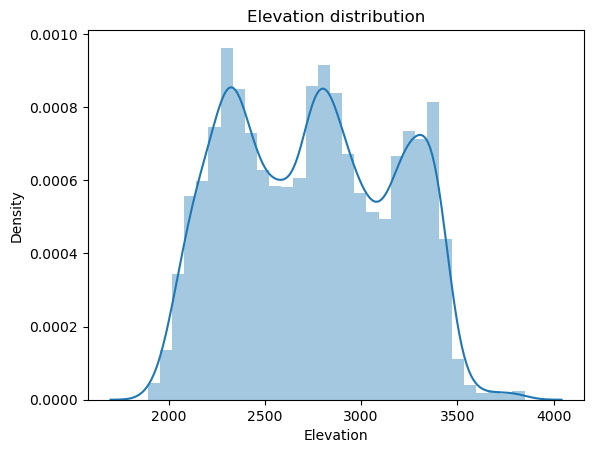
\includegraphics[width=0.4\textwidth]{elevation_distribution.png}
    \caption{Répartition de la variable \textit{Elevation} dans l'ensemble d'entraînement}
  \label{fig:elevation}
\end{figure}

La figure \ref{fig:elevation} montre par exemple la répartition de \textit{Elevation} dans le jeu d'entraînement. Les graphes des autres variables numériques sont fournis en annexe sur la figure \ref{fig:all_distributions}. Ces graphes ont été réalisés avant le scaling pour que la visualisation des données se fasse avec de vraies valeurs.

Nous avons vu que la variable \textit{Elevation} est discriminante pour permettre d'identifier le \textit{CoverType}, car à une élévation donnée, il y a souvent un \textit{CoverType} majoritaire. Les \textit{CoverType} 4, 5 et 7 sont notamment très facilement discriminables, comme on peut l'observer sur le graphe de la figure \ref{fig:elevation_per_covertype}, ou encore sur les boxplots de la figure \ref{fig:boxplot}.

\begin{figure}[h]
  \centering
  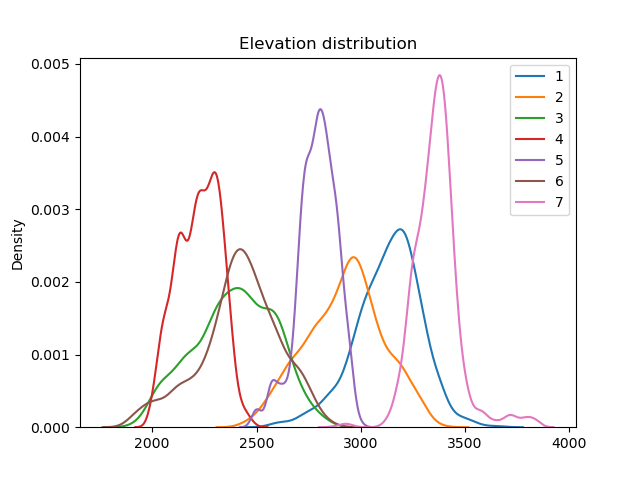
\includegraphics[width=0.45\textwidth]{Elevation_distribution2.png}
    \caption{Répartition de la variable \textit{Elevation} dans l'ensemble d'entraînement en fonction du \textit{CoverType}}
  \label{fig:elevation_per_covertype}
\end{figure}

\begin{figure}[h]
  \centering
  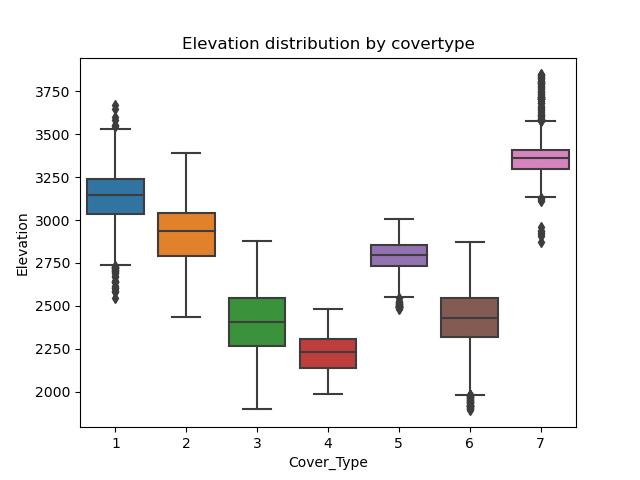
\includegraphics[width=0.45\textwidth]{Elevation_distribution_by_covertype.png}
    \caption{Boxplot de \textit{Elevation} par \textit{CoverType}}
  \label{fig:boxplot}
\end{figure}

Nous nous sommes ensuite intéressés à la distribution des données et aux relations entre celles-ci et \textit{CoverType}. Le graphe de la figure \ref{fig:corr} montre la valeur absolue du coefficient de corrélation entre les différentes variables et \textit{CoverType}. Cela nous permet d'observer quelles variables sont le plus liées au \textit{CoverType} pour optimiser le classifieur en enlevant du jeu de donnée les variables "inutiles" qui ne font que bruiter le signal d'entrée.

\begin{figure}[h]
  \centering
  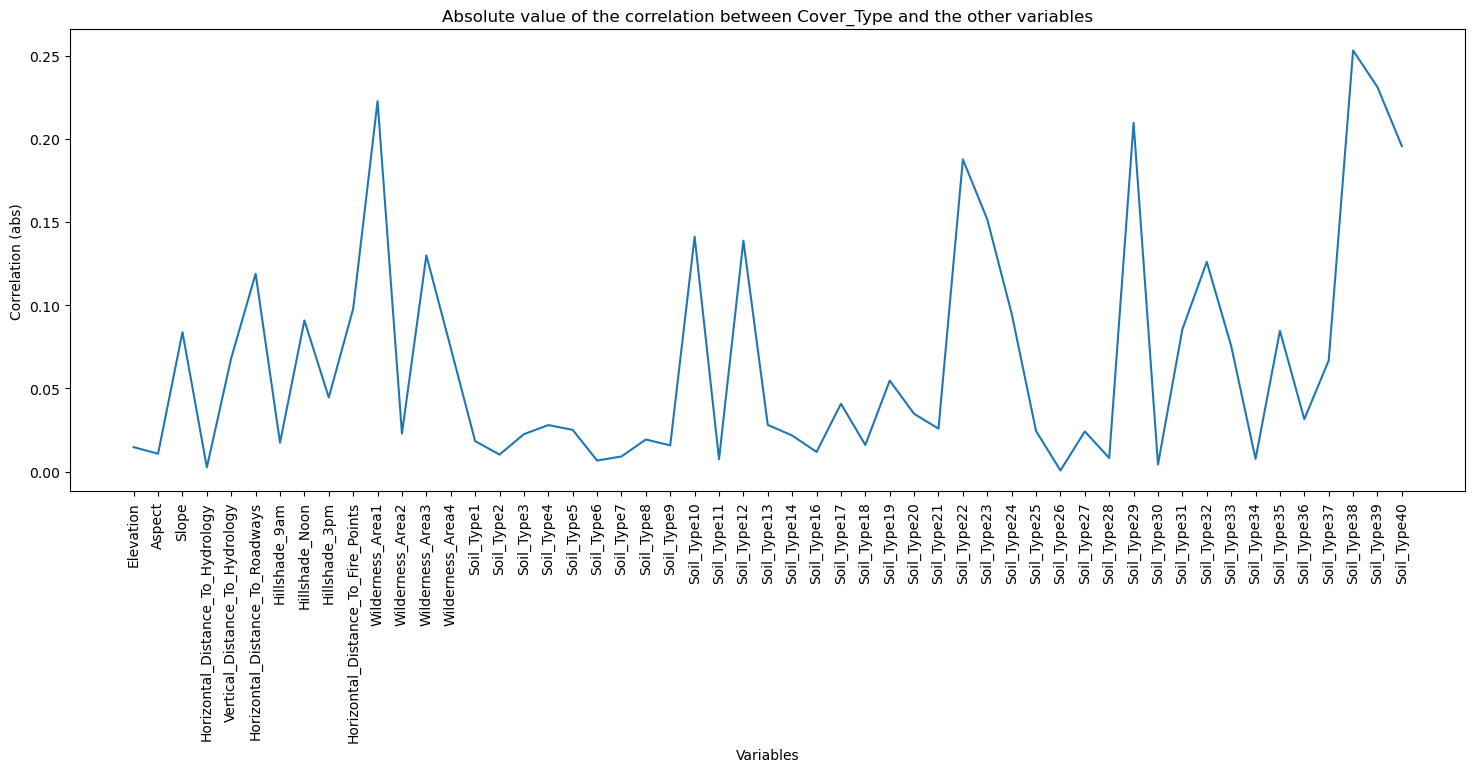
\includegraphics[width=0.6\textwidth]{correlation.png}
    \caption{Valeur absolue de la corrélation entre chacune des variables et \textit{CoverType}}
  \label{fig:corr}
\end{figure}

\newpage
\section {Pre-processing des données}

Il est parfois très utile de faire un pre-processing des données d'entraînement d'un algorithme pour optimiser sa performance. \textbf{Un jeu d'entraînement augmenté a ainsi été créé}, et nous avons entraîné différents algorithmes sur les deux jeux de données pour voir quelle combinaison algorithme / jeu d'entraînement donnait la meilleure performance.

Tout d'abord, nous avons normalisé les variables numériques dans les deux jeux de données pour éviter tout biais lié à l'échelle des valeurs et garantir une comparaison significative entre les différentes caractéristiques.

Nous n'avons ensuite plus touché au premier jeu de donnée et avons entraîné des algorithmes dessus. Nous avons augmenté le second en utilisant les données avec un sens physique: des combinaisons malines de celles-ci permettent d'obtenir de nouvelles données qui peuvent avoir un sens conduisant à l'amélioration des performances d'un algorithme.

Par exemple, nous avons créé une nouvelle variable numérique \textit{DistanceToHydrology} qui vaut :
\begin{equation}
    D_{hydro}=\sqrt{D_{vert\_hydro}^2 + D_{hor\_hydro}^2}
\end{equation}

Avec $D_{vert\_hydro}$ valant \textit{HorizontalDistanceToHydrology} et  $D_{hor\_hydro}$  valant \textit{VerticalDistanceToHydrology}.\\ Nous avons également créé \textit{DistanceToAmenities} qui est égal à la somme de \textit{HorizontalDistanceToFirePoints} et de \textit{HorizontalDistanceToRoadways}, ainsi que \textit{MeanHillshade}, qui vaut la moyenne des 3 valeurs \textit{Hillshade}. Nous avons aussi ajouté d'autres variables ayant un sens physique de la même manière.

Les variables \textit{SoilType} prenant beaucoup de place, nous avons décidé de les éliminer en partie. Des recherches nous ont montré que \textit{SoilType} est une classification prenant en compte d'autres caractéristiques telles que la zone géologique et climatique. Cette information étant plus forte que le \textit{SoilType}, nous avons supprimé la variable \textit{SoilType} et l'avons remplacée par les variables \textit{GeologicZone} et \textit{ClimaticZone}, ainsi que par d'autres variables représentant le \textit{SoilType}.\\
\textbf{La réduction des variables catégorielles permet d'éviter de s'encomber avec une structure très sparse}, et leur absence de sens physique les rend moins facile à interpréter que les variables numériques. 

Les différences entre le jeu de donné de base et préprocessé sont résumées dans le tableau \ref{tab:avant_après}

\begin{table}[h]
  \centering
  \begin{tabular}{|c|c|c|}
    \hline
     & Jeu de base & Jeu préprocessé \\
    \hline
    Variables numériques & 10 & 29 \\
    \hline
    Variables catégorielles & 44 & 21 \\
    \hline
  \end{tabular}
  \caption{Avant / Après pre-processing}
  \label{tab:avant_après}
\end{table}

\newpage

\section{Choix des modèles et performance}

\subsection{Choix des modèles}

Avec un dataset mélangeant des variables de différents types, nous avons considéré un large éventail de classifieurs, à savoir : 
\\
$\bullet$ Logistic Regression 
\\ $\bullet$ KNN : k nearest neighbor
\\ $\bullet$ SVM : Support Vector Machine 
\\ $\bullet$ Random Forest 
\\ $\bullet$ XGB 
\\ $\bullet$ Light GBM 
\\ $\bullet$ Extra Trees

\subsection{Premiers résultats}

\textbf{Sans chercher à optimiser les hyperparamètres, nous avons testé chaque modèle} sur le jeu normal et pré-processé avec des paramètres par défaut. 

Cette partie présente les premiers modèles que nous avons tentés d'étudier ainsi que les scores associés. La métrique que nous avons utilisée est la fréquence de bonne classification, qui nous est parue pertinente puisque c'est celle utilisée sur le leaderboard du challenge. Néanmoins, afin de mieux interpréter les erreurs, d'autres métriques telles que le F1-score peuvent être utilisées.

Les résultats sont résumés dans le tableau ci-dessous : 
\\

\begin{table}[h]
    \centering
    \begin{tabular}{|c|c|c|} \hline 
         Modèle&  Jeu de base& Jeu pré-processé\\ \hline 
         Logistic Regression&  0.62& 0.71\\ \hline 
         KNN&  0.82& 0.83\\ \hline 
         SVM&  0.54& 0.65\\ \hline 
         Random Forest&  0.87& 0.90\\ \hline 
         XGB&  0.87& 0.89\\ \hline 
         Light GBM&  0.86& 0.88\\ \hline 
         Extra Trees&  0.86& 0.90\\ \hline
    \end{tabular}
    \caption{Fréquence de bonne identification sur le jeu de validation pour chaque classifieur, hyperparamètres par défaut}
    \label{tab:my_label}
\end{table}

On peut constater de ces premiers tests que : 

$\bullet$  \textbf{Le jeu de données pré-processés permet d'améliorer systématiquement les résultats}, confirmant nos intuitions sur le rééquilibrage des variables et la recherche de nouvelles. Nous avons donc décidé de ne travailler plus que sur le jeu préprocessé, notamment pour l'optimisation des hyperparamètres. 

$\bullet$ \textbf{Les 4 derniers modèles (Random Forest, XGB, Light GBM et Extra Trees) performent beaucoup mieux} que les premiers modèles, il est trop tôt pour les exclure de nos tests mais ils semblent être de bons potentiels candidats pour nos prédictions finales.


\newpage

\subsection{Optimisation des hyperparamètres}

Chacun de ces modèles ayant des performances dépendant fortement de leurs hyperparamètres, nous avons ensuite cherché à les optimiser sur l'ensemble d'entraînement pre-processé, pour voir quelle combinaison de paramètres permettait d'arriver aux meilleures performances. Nous avons pour cela réalisé un \textbf{grid search}, en augmentant pas à pas les hyperparamètres pour chacun des modèles, avant de l'entraîner sur les deux jeux d'entraînement puis de tester les prédictions sur les jeux de validation. Encore une fois, une validation croisée a été réalisée pour augmenter la précision de nos chiffres.  \\ 

Le Grid Search performé a été le suivant : 
\\


\begin{table}[h]
\centering
\begin{tabular}{|c|c|c|c|c|c|}
\hline
Modèle & Paramètres & Valeurs &  Valeure  & Fréquence \\
\hline
Logistic Regression & C & [0.01, 0.1, 1, 10, 100] & 100 & 0.71 \\
 & Penalty & ['l1', 'l2'] & L2 & \\
 & Solver & ['liblinear', 'saga', 'lbfgs', 'newton-cg'] & saga & \\
\hline
K Nearest Neighbors & n\_neighbors & list(range(5, 20)) & 5 & 0.83 \\
 & leaf\_size & [5, 10, 20, 30, 40] & 5 & \\
 & weights & ['uniform', 'distance', 'ball\_tree', 'kd\_tree'] & distance & \\
\hline
Support Vector Machine & C & [0.01, 0.1, 1, 10, 100] & 100 & 0.78 \\
 & Kernel & ['linear', 'poly', 'rbf', 'sigmoid'] & rbf & \\
 & Gamma & ['scale', 'auto'] & scale & \\
\hline
Random Forest & n\_estimators & [100, 200, 300, 400, 500] & 400 & 0.896 \\
 & max\_depth & [5, 10, 15, 20, 25, 30] & 30 & \\
 & min\_samples\_split & [2, 5, 10, 15, 20] & 2 & \\
 & min\_samples\_leaf & [1, 2, 5, 10, 15, 20] & 1 & \\
\hline
XGBoost & n\_estimators & [100, 200, 300, 400] & 300 & 0.891 \\
 & max\_depth & [5, 10, 15, 20, 25, 30] & 10 & \\
 & learning\_rate & [0.01, 0.1, 0.2] & 0.2 & \\
 & gamma & [0, 0.1, 0.5, 1] & 0 & \\
\hline
LightGBM & n\_estimators & [50, 100, 200, 400] & 400 & 0.900 \\
 & max\_depth & [2, 4, 8, 16] & 16 & \\
 & learning\_rate & [0.01, 0.1] & 0.1 & \\
 & num\_leaves & [16, 32, 48, 64] & 64 & \\
\hline
Extra Trees & n\_estimators & [50, 100, 200, 250, 400]& 250 & 0.904 \\
 & max\_depth & [5, 10, 20, None] & None & \\
 & min\_samples\_split & [1, 2, 4, 8] & 2 & \\
 & min\_samples\_leaf & [1, 2, 4, 8] & 1 & \\
 & max\_features & ['auto', 'sqrt', 'log2'] & sqrt & \\
 & criterion & ['gini', 'entropy'] & gini & \\
\hline
\end{tabular}
\caption{Grid Search et paramètres retenus avec leur fréquence}
\label{tab:my_label}
\end{table}

\newpage

On peut voir sur le tableau \ref{tab:my_label} que les meilleurs performances sont atteintes par LightGBM et ExtraTrees entraînés sur le jeu d'entraînement pre-processé. Néanmoins, LightGBM est très lent à entraîner et performe légèrement moins bien que ExtraTrees. Nous avons donc décider de prendre \textbf{ExtraTrees comme modèle final}. 



\section{Résultats finaux et analyses}

Ainsi, le classifieur atteignant les meilleurs résultats en validation croisée est l'\textbf{Extra Tree Classifier}, avec les paramètres suivants:  \textit{n\_estimators=250, criterion='gini', max\_depth=None, min\_samples\_leaf=1, min\_samples\_split=2, max\_features='sqrt'. } \\


Il obtient une fréquence de bonne identification de \textbf{0.82606 sur le test\_set donné par le leaderboard du Kaggle}. 


Dans le cadre de la classification binaire, la métrique utilisée est rarement la fréquence de bonne identification. En effet, dans le problème de détection, une erreur consistant à mal classifier une instance de la classe positive (faux négatif) peut avoir des conséquences plus graves que de mal classifier une instance de la classe négative (faux positif), par exemple lors de la détection d'un piéton par une voiture autonome ou d'un cancer sur une radiographie. Par conséquent, d'autres métriques peuvent être utilisées, comme la précision ou le rappel et permettent ainsi de donner les marges de progression d'un algorithme ou encore d'accompagner un résultat de sa fiabilité. \\

Dans notre cas, il ne s'agissait pas de détection mais bien de classification avec 7 résultats possibles pour chaque donnée. Pour évaluer les performances de notre classifieur sur chaque \textit{CoverType}, nous avons entraîné Extra Tree sur 80\% du jeu d'entraînement et testé sur les 20\% restants. Nous avons ensuite calculé la précision, le rappel et le F1-score associés à chaque \textit{CoverType}. Pour cela, nous avons associé à chaque \textit{CoverType} dans ${1, ... 7 } $ un vecteur de détection de la manière suivante: \\
$ \forall i \in {1, ..., 7}, y_{i, pred}(j)= \mathbb{1}_{y_{pred}(j)=i}$ avec $y_{i, pred}$ le vecteur de détection associé au \textit{CoverType} $i$ et $y_{pred}$ le vecteur de classification. 

Nous avons ensuite calculé la précision, le rappel et le F1-score associés qui sont résumés dans le tableau \ref{tab:cover_metrics}





\begin{table}[h]
  \centering
  \begin{tabular}{|c|c|c|c|}
    \hline
    Cover Type & Precision & Recall & F1 Score \\
    \hline
    1 & 0.826 & 0.845 & 0.836 \\
    \hline
    2 & 0.874 & 0.763 & 0.815 \\
    \hline
    3 & 0.906 & 0.895 & 0.901 \\
    \hline
    4 & 0.955 & 0.982 & 0.968 \\
    \hline
    5 & 0.915 & 0.971 & 0.942 \\
    \hline
    6 & 0.894 & 0.916 & 0.905 \\
    \hline
    7 & 0.963 & 0.972 & 0.968 \\
    \hline
  \end{tabular}
  \caption{Précision, Rappel, et F1 Score pour différent Different \textit{CoverType}}
  \label{tab:cover_metrics}
\end{table}

Ce tableau permet d'avoir une profondeur nouvelle sur les prédictions de notre algorithme: ainsi, le \textit{CoverType} obtenant la meilleure précision est le 7, ce qui signifie qu'il y a très peu de forêts labellisés 7 qui ne le sont pas réellement (il y a peu de faux positifs). A l'inverse, le \textit{CoverType} avec le meilleur rappel est le 4, ce qui veut dire que le \textit{CoverType} le moins raté par notre algorithme est le 4 (peu de faux négatifs): si on fait une prédiction sur un ensemble de forêts, quasiment toutes les forêts de type 4 seront dans la classe des 4 (il y aura par contre peut-être par contre des forêts d'autres types qui seront labellisées comme 4). \\

Cette analyse \textbf{permet à l'utilisateur de notre algorithme d'avoir un regard critique sur les résultats fournis} par celui-ci lors de son utilisation. 




\newpage

\section{Annexe}

\subsection{Figures}




\begin{figure}[h]
  \centering
  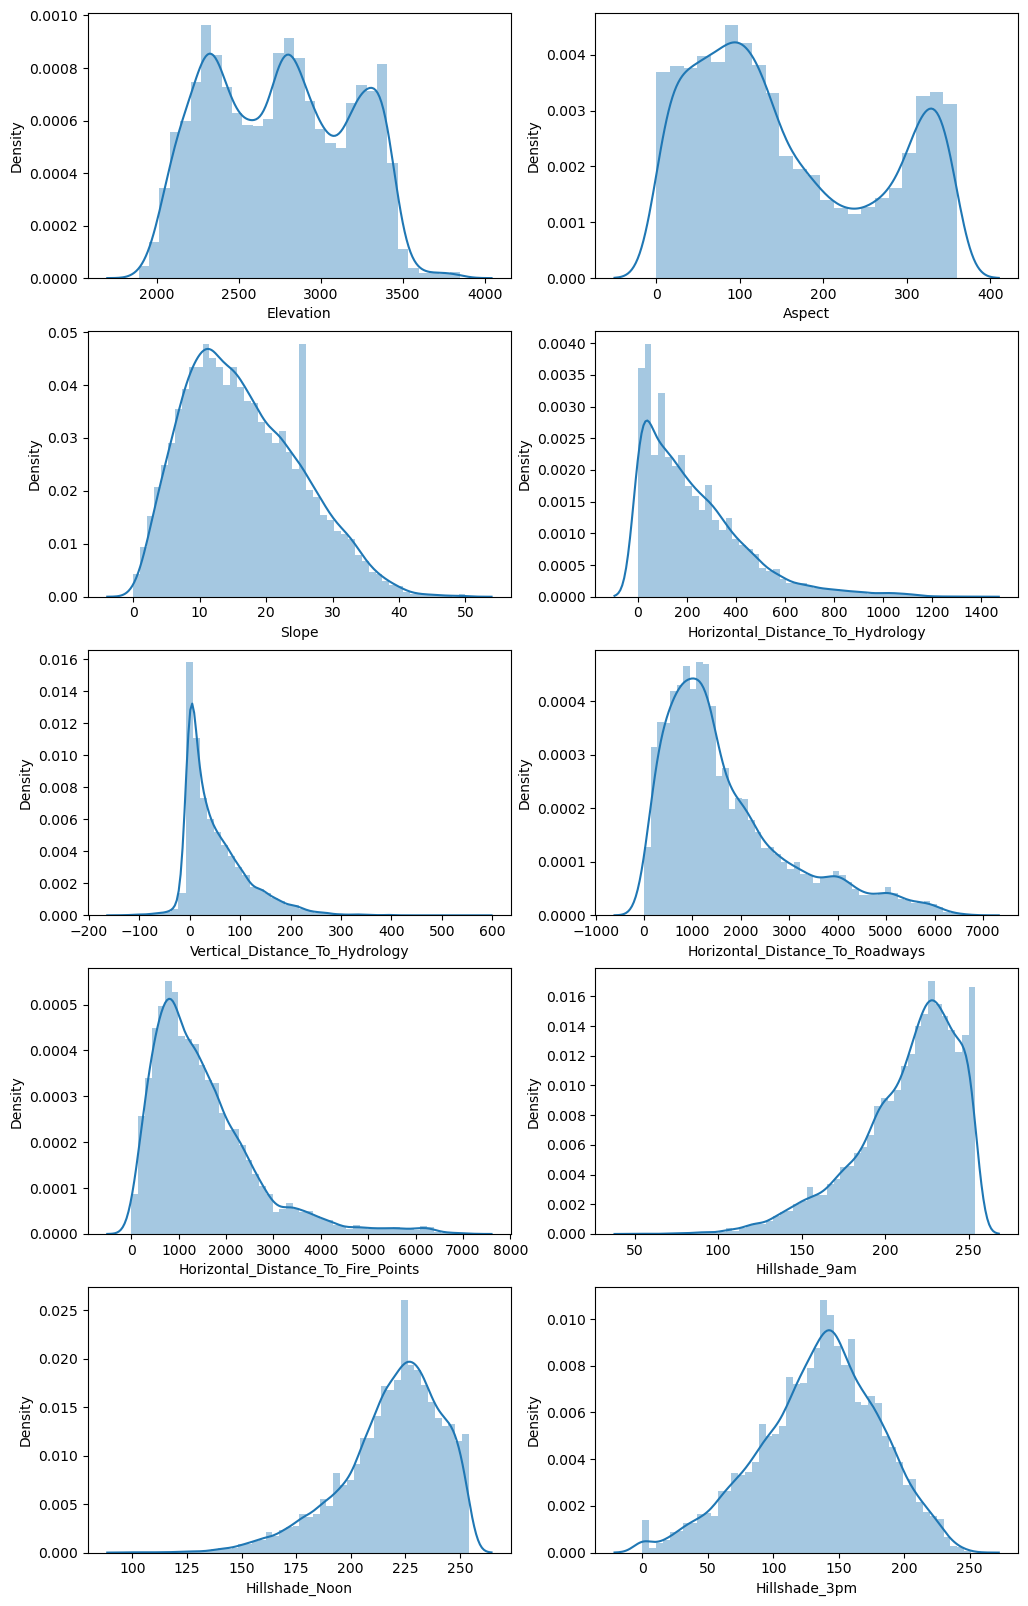
\includegraphics[width=0.6\textwidth]{all_distributions.png}
    \caption{Répartition des variables numériques dans l'ensemble d'entraînement}
  \label{fig:all_distributions}

  \end{figure}





\newpage
\begin{figure}[h]
  \centering
  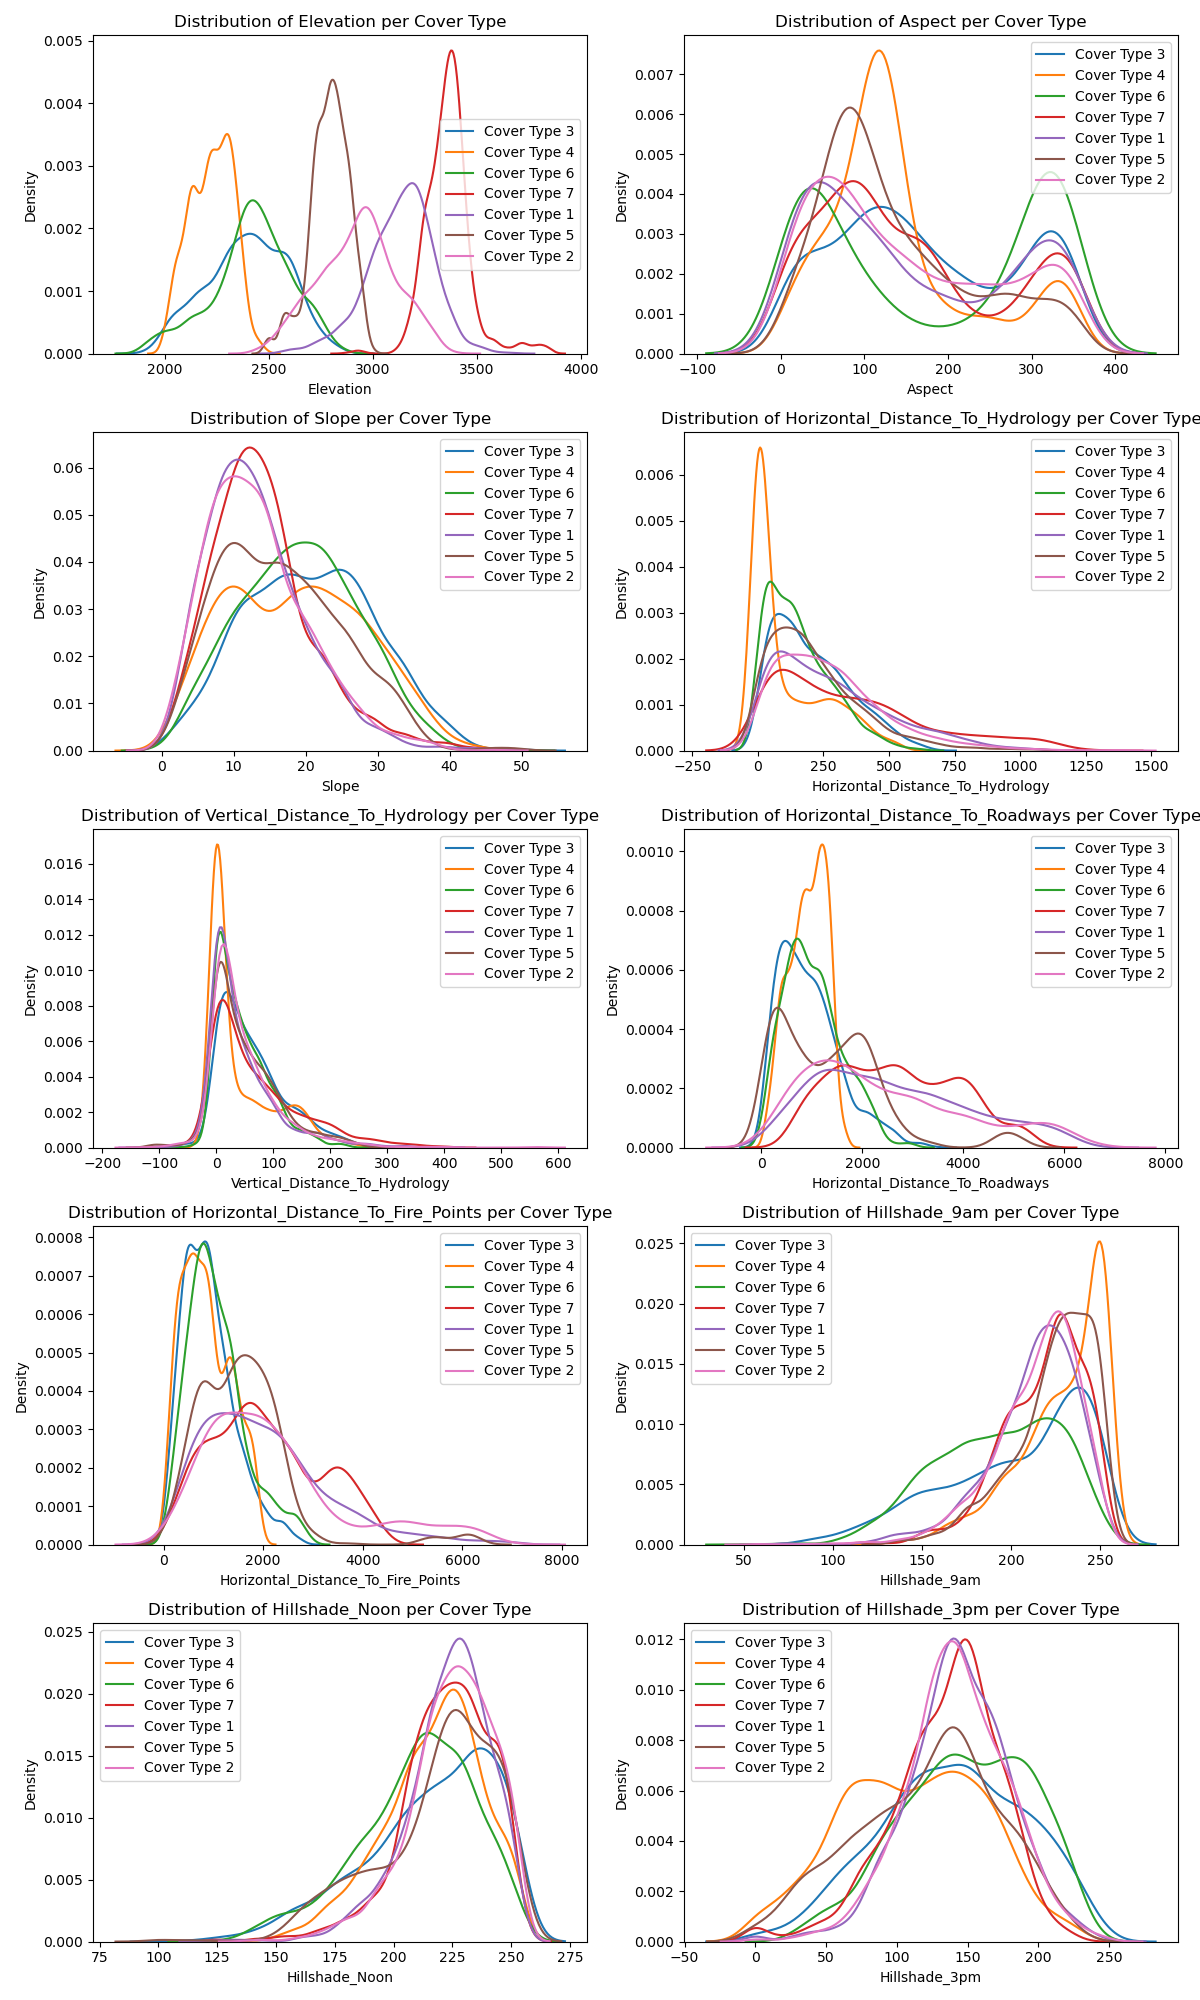
\includegraphics[width=0.6\textwidth]{numerical_variables_distribution.png}
    \caption{Répartition des variables numériques en fonction du \textit{CoverType}}
  \label{fig:varnumparcovertype}
\end{figure}
\newpage
\begin{figure}[h]
  \centering
  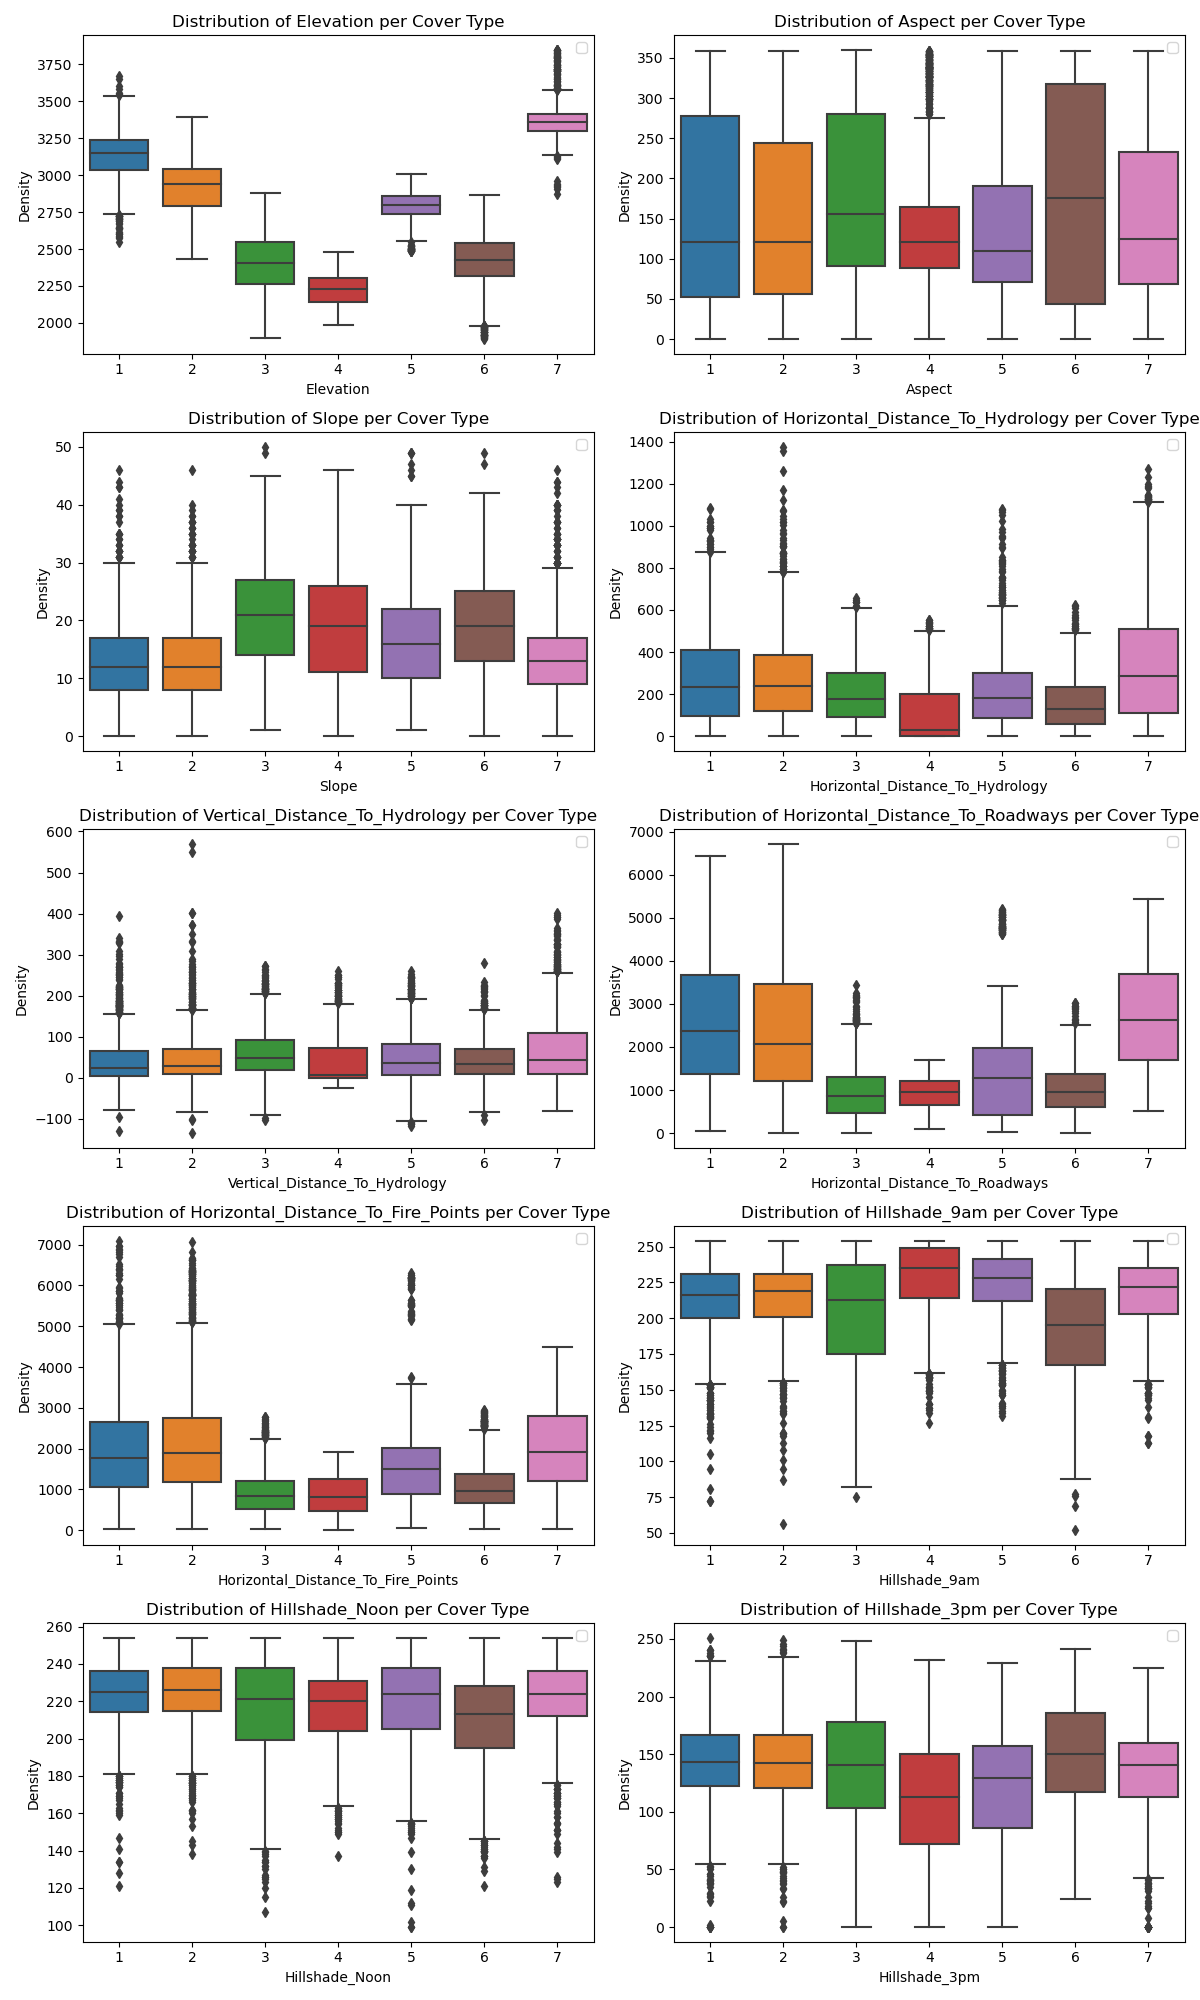
\includegraphics[width=0.6\textwidth]{numerical_variables_boxplot.png}
    \caption{Boxplot de toutes les variables numériques en fonction du \textit{CoverType}}
  \label{fig:boxplot_numerique}
\end{figure}
\newpage

\end{document}


